\section{Results and Discussion} 

	The main objective of this work is to explore the capability of an application of the Maximum Entropy ($MaxEnt$) framework to the modeling of the cellular metabolism in a continuous cultivations regime. $MaxEnt$ has been used for the analysis of other biology related problems with success. It has become into an useful tool when we are dealing with limited data, which actually is a common scenario in biology \shortcite{de_martino_introduction_2018}. In particular, the framework proposed in \shortcite{fernandez-de-cossio-diaz_characterizing_2017} and \shortcite{fernandez-de-cossio-diaz_maximum_2019} allows to link effectively the macroscopic variables that defined the state of a chemostat steady state, commonly accessible, with the underlying cellular metabolic state, harder to determine. 
	
	In the former article, a more traditional approach to model the metabolism was taken. It delegates in Flux Balance Analysis ($FBA$) \shortcite{orth_what_2010} for choosing the vector of reactions fluxes assumed to be determining the current metabolic state of the cell under the cultivation conditions. This method have been heavily used in the past decades with good results and a variety of applications ($citeRequired!!!$). 
	It has the advantage of not requiring kinetic parameters from the cellular metabolism, which are generally unavailable data.
	This is possible because $FBA$ apply a steady state assumption, justified in the time scale difference between regulatory (slow) and metabolic (fast) processes \shortcite{de_martino_introduction_2018}. 
	Another assumption $FBA$ makes is that the cell population in the culture is homogeneous and are optimizing a given metabolic objective. 
	$FBA$ returns the vector of all reactions fluxes that optimize the objective function subject to the applied constraints ($citeRequired!!!$). 
	This vector will be taken as the definition of the metabolic state for all the cells in the culture, and with it all the predictions or analysis will be made \shortcite{fernandez-de-cossio-diaz_characterizing_2017}. 
	
	To overcome the limitation of not considering culture heterogeneity, although data shows that two cells in a culture are unlikely to be equal ($[citeRequired!!!18, ]$), a probability distribution can be defined over the set of all the possible metabolic states.
	This distribution describe how probable a cell is found in one of the those states.
	To infer such probability distribution in agreement with available experimental data, the $MaxEnt$ principle can be used  \shortcite{fernandez-de-cossio-diaz_maximum_2019}. 
	Precisely, in this work $MaxEnt$ was apply in such a way that it returns the probability distribution that maximized the entropy and ensure the expected value of the growth rate to match with the experimentally observed.
	Now, instead of a vector of reactions fluxes that optimize an objective function, the model will returns a vector containing the expected values for each reaction flux due to the inferred $MaxEnt$ distribution. 
	This is a major advantage with respect to the $FBA$ framework, $MaxEnt$ do not assume that the cells $"have\ a\ goal"$, an objective function, it claims to compute the bias-less probability distribution in concordance with the imposed, data driven, constraints \shortcite{de_martino_introduction_2018}. 
	The predictions of $FBA$ based on the optimization hypothesis 
	
	
	\subsubsection{Human}
	
		 	\begin{figure}[H]
		 	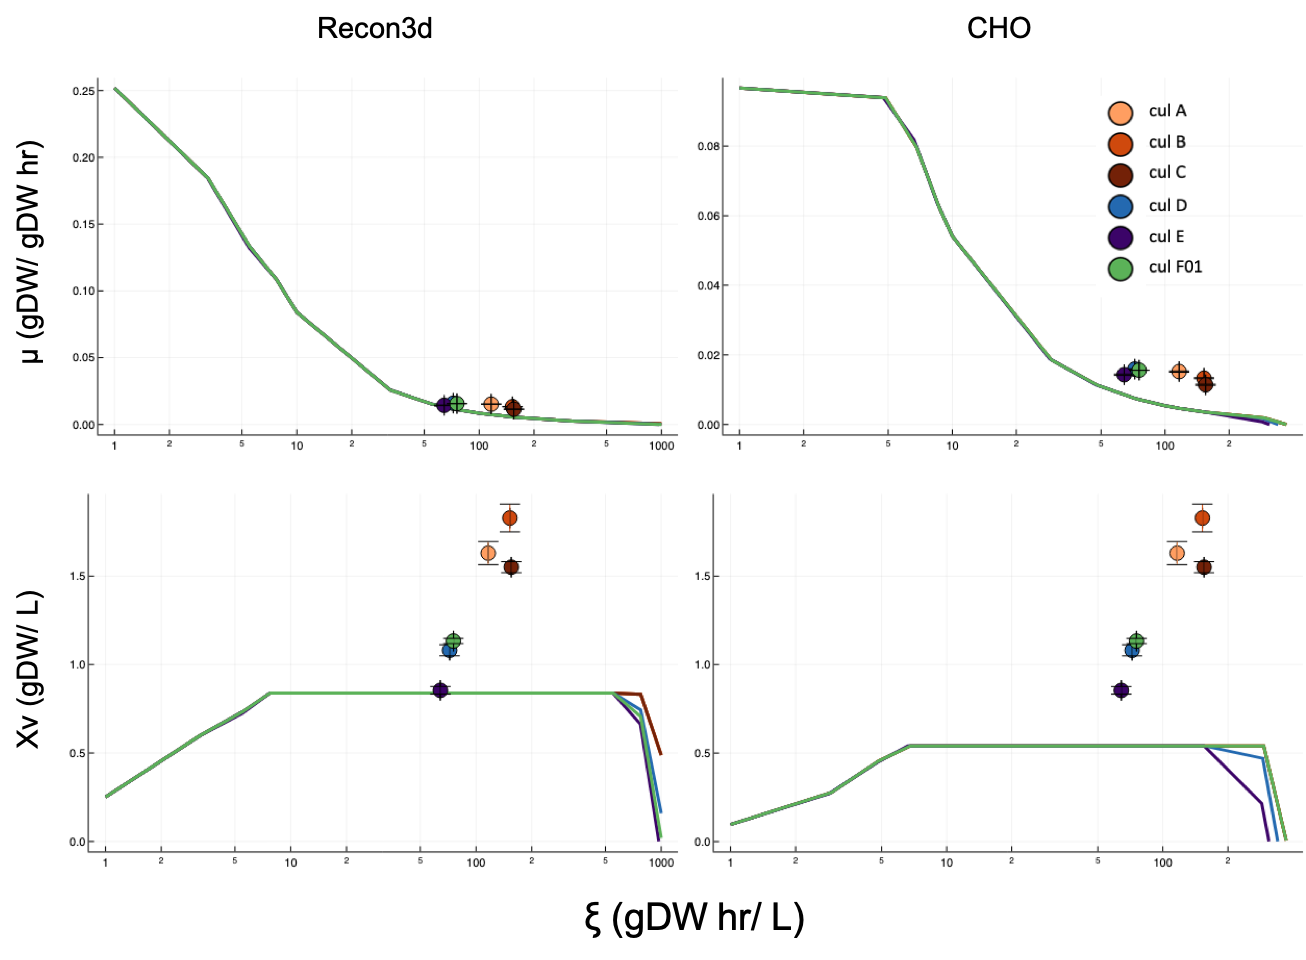
\includegraphics[scale = 0.5]{low_medium_1}
		 	\caption{$FBA$ results showing the growth rate, $\mu$, and the viable cell density, $Xv$, dependence of $\xi$ for the six steady states. The solid lines represent the model predictions and the colored points show the experimental results. The model data was obtained for feed mediums with 0.5mM ($Recon3D$) and 0.0mM ($CHO$) concentration of phosphatidylethanolamine}
		 	
		 \end{figure}
		
		
%  	\subsection{Low concentrations of phosphatidylethanolamine} 
	
	Because phosphatidylethanolamine isn't a reported component of the 42-Max-UB-medium, $Tabla\ 1$, and it can be a carbon source for the GEMs, its concentration was set first to the lowest value possible. For Recon3D it was fixed to 0.1mM, a handpicked value, and for CHO it wasn't present in the feed medium at all.
	
	Flux balance analysis with molecular crowding (FBA) was performed similarly to \cite{Fernandez-de-Cossio-Diaz2018b}. Plots of $\mu$ and $Xv$ as a function of $\xi$ are shown in $Figure\ 1$. Both networks failed to reach the experimental values for both observables. In the case of $Xv$, in all the explored $\xi$ range (from 1 to 1000 gDW hr/ L) the value was underestimated. This result may have several causes. One could be that the GEM have a "too expensive" biomass equation. We mean that one or more biomass required precursors might be overestimated. However, this reason seems hard to sustain because we modified Recon3D biomass equation with the reported anabolic biomass demand for AGE1.HN.AA1 \cite{Niklas2013}. We use the reported anabolic demand of proteins, lipids, DNA, RNA and carbohydrates to fix the total demand of this same groups in the original Recon3D biomass equation and the changes wasn't too big. For CHO we kept the biomass equation unmodified. Nonetheless, a modification in the biomass equation would be an elegant way to solve the problem. Other plausible cause could be a big difference between the models frameworks. But, both works model the chemostat in an equivalent fashion, as can be seen when comparing equations 1 with 3.25 and 2 with 3.28 and 3.29 from \cite{Fernandez-de-Cossio-Diaz2017} and \cite{Rath2017a} respectively.
	 
	Moreover, other parameter than can affect $Xv$ is the bleeding coefficient, $\phi$,
	defined in perfusion systems as the fraction of cells that escape from the culture through a cell-retention device \cite{Fernandez-de-Cossio-Diaz2017}. Because, \cite{Rath2017a} doesn't report the use of any retention devise in the cultures this parameter was taken as 1.0, but lower values will cause to increment the predicted value of  $Xv$ by the model. Finally, it needs to be taken into consideration that we are using GEMs that are not directed curated for the working cell line. This is, by far, the most difficult factor to solve, because the curing of a genome scale metabolic network is a very laborious labor.

	
	On other hand, correlations of experimental and modeled uptakes, $Figure\ 2$, was performed. The graphs shows better results for the uptakes of $GLC$ and $GLN$, 
	and worse correlations for uptakes such as $PYR$, $NH4$ and $LAC$ for both GEMs. In general, CHO had better correlations than Recon3D. This could be, maybe, explained because Recon3D is a general GEM, allowing the model to access to all the possible genome repertory present in humans, a fact that is not accurate for a cell in the $in\ vivo$ scenario. Additionally, CHO was curated for a defined cell line, representing a more restricted and realistic network. Anyway, it is remarkable that the models reproduce uptakes like $GLC$ and $GLN$ regarding all the previous consideration.
%	\subsection{High concentrations of phosphatidylethanolamine}

	To avoid the undesired $Xv$ and $\mu$ underestimation, a less realistic scenario was considered. An extra carbon source was put in excess in the feed medium. We select the phosphatidylethanolamine ($PE$) because it was already introduced in the $Recon3D$ medium, do to the incapacity of this GEM to growth without this (or similar) metabolite, and it is an usable carbon source. So, the feed medium concentration of	$PE$ was set to a high value, 20 mM (a handpicked value), for both GEMs. 
 	
 		\begin{figure}[H]
		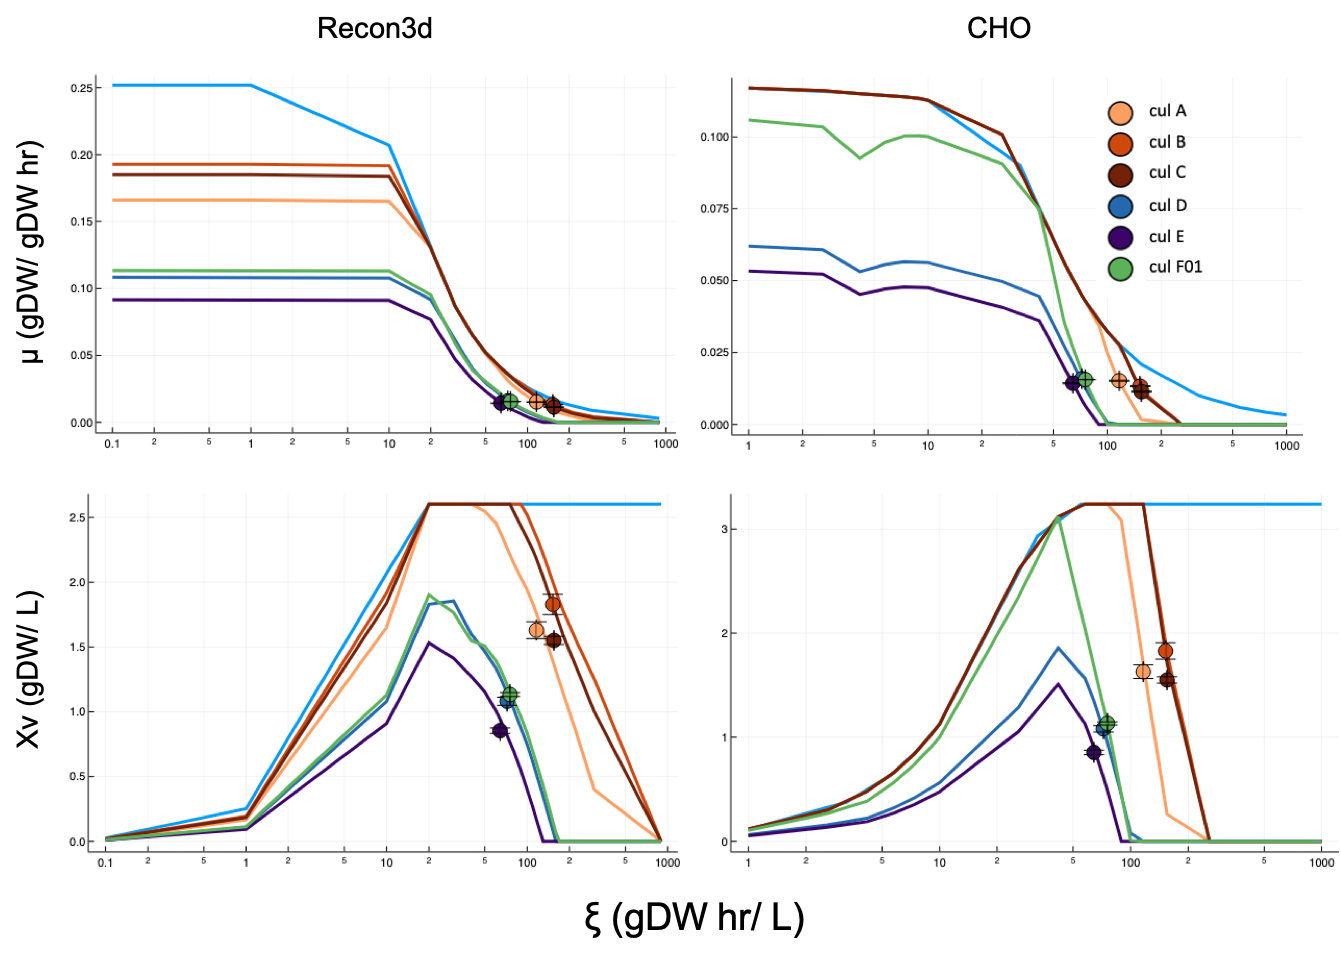
\includegraphics[scale = 0.5]{rich_medium_1}
		\caption{$EP$ and $FBA$ results showing the growth rate, $\mu$, and the viable cell density, $Xv$, dependence of $\xi$ for the six culture conditions. The solid lines represent the model predictions and the color points show the experimental results. $FBA$ results are shown as the solid light blue line. $EP$ $\beta$ parameters was chosen, for each culture, so that the experimental $\mu$ coincides with the modeled one}
		
	\end{figure}
 	
 	This time, additionally to $FBA$, the expected propagation ($EP$) algorithm was used to introduce a population heterogeneity factor \shortcite{Fernandez-de-Cossio-Diaz2018b}. $Figure\ 3$ shows the results of both methods for $Recon3D$ and $CHO$. As can be appreciated, FBA (lite blue solid line) overestimate the experimental results. This is consistent with the fact that we put a carbon source, $PE$, in a high concentration, allowing the network to reach higher $\mu$ and $Xv$ values.
 	
 	 	\begin{figure}[H]
		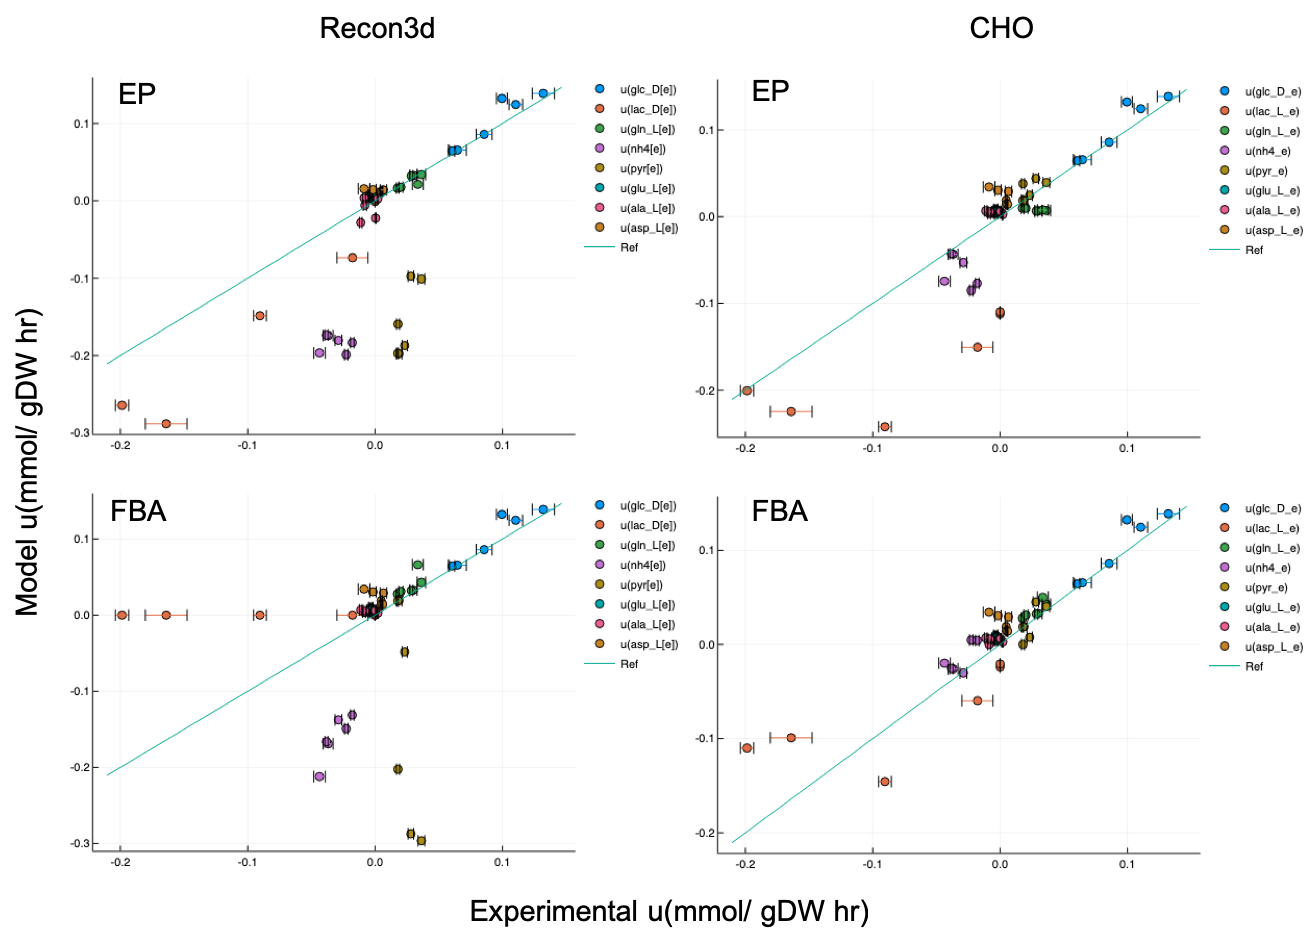
\includegraphics[scale = 0.5]{rich_medium_2}
		\caption{Correlations of all the experimental uptakes compared with the predicted value from $EP$ and $FBA$ for $GEMs$ with 20mM concentration of phosphatidylethanolamine.}
		
	\end{figure}


 	
  	On the other hand, $EP$ can be tuned through parameter $\beta$. This parameter can be interpreted as a measurement of the cell heterogeneity in the culture \shortcite{Fernandez-de-Cossio-Diaz2018b}. $\beta$ values closer to zero indicate higher heterogeneity in the culture, or that the cells can explore more uniformly the space of possibles metabolic states. By contrast, larger $\beta$ values will be approaching the $EP$ model result to $FBA$ result, meaning that no cell heterogeneity is accounted at all. As is appreciated in $Figure\ 3$, considering different $\beta$ values allow the $EP$ model to reproduce the measured $\mu$ and $Xv$. This is an interesting result for several reasons. First, it improves the $FBA$ solution. $FBA$ is insensible to the different experimental conditions, as shown in $Figure\ 1\ and\ 3$. This means that it does not vary the observable predictions, mainly $Xv$, after changing the particular culture conditions, metabolite feed medium concentrations and dilution rate. This occurs for both situations, low and high concentration of $PE$, at least with this $GEM$s and settings. This could, maybe, be explained because $FBA$, as used in this work, returns an optimal metabolic state that maximizes $\mu$. However, it is possible that many different states maximize $\mu$, a not unique solution scenario, and this can make the network robust enough to be insensible to the changes in the input. 
  	
  	Because $EP$ introduces the heterogeneity factor, a better exploration of the space of feasible metabolic states is now possible. There are many factors that can influence the heterogeneity of a population of cells \shortcite{Elowitz2002, Tzur2009, Huh2011, Delvigne2014, King2016, Wang2016, Gonzalez-Cabaleiro2017,  Fernandez-de-Cossio-Diaz2019}. The experimental results can be then interpreted, not only because different input conditions lead to an unique different metabolic state, but because these same changes in the input modified the likelihood distribution of the feasible metabolic states through the cell population. This interpretation is qualitatively different from what $FBA$ represents.
	
  	Furthermore, the correlation of experimental and modeled uptakes was performed, $Figure\ 4$, for both methods. Again, the best correlations were achieved for the uptakes of $GLC$ and $GLN$. A small improvement in the general results can be observed for $EP$ compared with $FBA$, in particular for $Recon3D$. The causes that are driven these results could be the same disused in the previous section. 